%(BEGIN_QUESTION)
% Copyright 2010, Tony R. Kuphaldt, released under the Creative Commons Attribution License (v 1.0)
% This means you may do almost anything with this work of mine, so long as you give me proper credit

Calculate all voltages, currents, and total power in this balanced Y-Y system:

$$\includegraphics[width=15.5cm]{i02421x01.eps}$$

\begin{itemize}
\item{} $E_{line} =$
\vskip 10pt
\item{} $I_{line} =$
\vskip 10pt
\item{} $E_{phase(source)} =$
\vskip 10pt
\item{} $I_{phase(source)} =$
\vskip 10pt
\item{} $E_{phase(load)} =$
\vskip 10pt
\item{} $I_{phase(load)} =$
\vskip 10pt
\item{} $P_{total} =$
\end{itemize}

\vfil 

\underbar{file i02421}
\eject
%(END_QUESTION)





%(BEGIN_ANSWER)

This is a graded question -- no answers or hints given!

%(END_ANSWER)





%(BEGIN_NOTES)

Important concepts to keep in mind when analyzing three-phase networks is that of {\it series} and {\it parallel} connections: series-connected components must always share the same amount of current, while parallel-connected components must always share the same amount of voltage.  This is why line current and phase current are identical in wye networks: because each phase element is directly in series with each line conductor.  This is why line voltage and phase voltage are identical in delta networks: because each phase element is directly in parallel with a pair of line conductors.

\vskip 10pt

\begin{itemize}
\item{} $E_{line} =$ 479.8 V
\item{} $I_{line} =$ 0.478 A
\item{} $E_{phase(source)} =$ 277 V
\item{} $I_{phase(source)} =$ 0.478 A
\item{} $E_{phase(load)} =$ 277 V
\item{} $I_{phase(load)} =$ 0.478 A
\item{} $P_{total} =$ 396.9 W
\end{itemize}

%INDEX% Electronics review: 3-phase voltage/current/power calculation

%(END_NOTES)



